\documentclass[a4paper, 12pt]{report}
\usepackage[a4paper, top=2.5cm,bottom=2cm,left=2cm,right=2cm]{geometry}
\usepackage[utf8]{inputenc}
\usepackage[T1]{fontenc}
\usepackage[italian]{babel}
\usepackage{lmodern}
\usepackage{verbatim}
\usepackage{csquotes}
\usepackage{subcaption}
\usepackage{graphicx}
\DeclareGraphicsExtensions{.png}

\begin{document}

%PRIMA PAGINA
\begin{titlepage}
  \begin{center}
    \LARGE{PROGRAMMAZIONE PER L'INTERNET OF THINGS A.A 2021/2022} \\
    \vspace{9cm}
    \Huge{Smart Box IoT}
  \end{center}
  \vspace*{\fill}
  \begin{flushright}
    \large{\textbf{Studente:} Lorenzo Calisti} \\
    \large{\textbf{Matricola:} 307458}
  \end{flushright}
  \vspace{1cm}
  \begin{center}
Questa relazione è stata preparata utilizzando \LaTeX
  \end{center}
\end{titlepage}

%\part* {\textit {Sezione}}
\subsection*{Introduzione}
\vspace{0.5cm}

Per questo progetto si è scelto di realizzare una "Smart Box" IoT focalizzata all'agricoltura. 

In questi anni si sente sempre più parlare della minaccia del cambiamento climatico e di come esso affliggerà le vite di tutta la popolazione mondiale in un futuro non troppo lontano, per questo motivo è fondamentale 
un cambio di mentalidtà da parte di tutte le industrie volto all'utilizzo di energie rinnovabili e alla creazione di nuovi metodi produttivi in modo da ridurre i consumi, le emissioni e l'inquinamento globale.

Secondo i maggiori esperti la tecnologia avrà un impatto decisivo nella vittoria della "guerra" contro il cambiamento climatico; il suo ruolo è quello di supporto, ottimizzndo i vecchi processi produttivi
e aiutando la scoperta di nuovi metodi di produzione più eco sostenibili con meno sprechi e consumi.
Nel campo dell'agricoltura l'utilizzo della tecnologia come supporto alla produzione sta prendendo piede da diversi anni, il problema principale è l'elevato costo che la rende accessibile solo da aziende di grandi dimensioni.

Il tipo di tecnologia più comune in ambiente agricolo è la "centralina meteo", se posizionata fra i campi consente di raccogliere continuamente dati sulle attuali condizioni atmosferiche e sulla qualità del terreno in modo
da sapere quale sia il miglior momento per irrigare, riducendo lo spreco d'acuqa, capire se è arrivato il momento del raccolto, evitando la raccolta di prodotti non ancora pronti, e addirittuta prevedere piogge o 
periodi di siccità futuri, in modo da prepararsi preventivamente ad essi.

La raccolta passiva dei dati è un tipo di tecnologia utilizzato dalle grandi industrie da più di quarant'anni, il vero elemento innovativo è l'utilizzo dell'IoT. L'internet of things, IoT in breve, rappresenta l'unione del
mondo reale, le cose, con il mondo vistruale, la rete internet; il suo scopo è quello di connettere fra loro tutti i sistemi fisici di raccolta dei dati dandogli un "cervello". Citando il cretore dell'IoT Kevin Ashton: 

\begin{displayquote}
  In the twentieth century, computers were brains without senses - they only knew what we told them. In the twenty-first century, because of the Internet of Things, computer can sense things for themselves
\end{displayquote}

La "Smart Box" IoT creata per questo progetto tiene bene a mente tutte queste idee; la sua funzionalità principale è quella di raccogliere dati sulla qualità dell'ambiente circostante in maniera continuativa per poi 
elaborarli "sul posto" e rilevare eventali anomalie che sono poi segnalate ad un sistema di monitoraggio remoto. Per fare questo si è partiti dalla progettazione e relizzazione del'hardware, per poi passare alla raccolta
di i dati "raw" e finire con l'addestramento di un modello di machine learning in grado di rilevare le anomalie dai dati che è poi stato installato nella Smart Box.
Di seguito vedremo più nel dettaglio tutte queste fasi con l'aggiunta di un analisi statistica sui dati raccolti inizialmente e sulle anomalie rilevate.

\subsection*{Progettazione Smart Box}
\vspace{0.5cm}

La "Smart Box" IoT, come dice il suo nome, è una scatola intelligente, con al suo interno una serie di sensori e un MCU impostati per raccogliere i dati una volta ogni 15 minuti. L'intera scatola è stata progettata 
per essere montata su un palo in modo da rimanere sempre sollevata dal terreno, il che è l'ideale per l'installazione in un campo dove, con la cresita delle colture, rischia di non essere più del tutto visibile.

Vediamo ora nel dettaglio tutti i componenti presenti all'interno della "Smart Box". Il più importante è senza dubbio l'MCU ESP8266, è il cuore dell'intero sistema, un chip a basso costo con Wi-Fi integrato e diversi pin
GPIO, molto popolare nelle applicazioni IoT.
Nella "Smart Box" sono stati inseriti i seguenti sensori:

\begin{itemize}
\item DHT11, sensore di temperatura e umidità
\item Sensore di rilevamento della pioggia 
\item YL-69, sensore igrometro per il rilevamento dell'umidità del terreno
\item MQ-135, sensore per il monitoraggio qualità dell'aria
\item LDR, sensore di luminosità 
\item BMP180, sensore combinato di temperatura, pressione e altitudine
\end{itemize}

Olre a questi componenti all'interno della scatola è stato inserito anche un LED di colore giallo utilizzato per segnalare lo stato del programma ed evantuali errori; infine, per alimentare l'MCU e tutti i sensori si 
è optato per la soluzione più semplice: un powerbank portatile con uscita a 5V, in questo modo non solo si evitano i diversi problemi dovuti alla gestione delle batterie LiPo, ma anche la ricarica è più 
facile e sicura, utilizzando un semplice caricatore per smartphone.

Una volta scelti tutti i componenti il primo passo per la progettazione della Smart Box è quello di realizzare delle schematiche che mostrino i diversi collegamenti elettrici fra loro; la Figura \ref{fig:schematics} 
e la Figura \ref{fig:breadboard} mostrano proprio questi schemi che sono stati fondamentali durante la fase di costruzione per tenere traccia di tutti i collegamenti elettrici. Questi diagrammi sono stati realizzati 
utilizzando Fritzing: un programma open source per la proggettazione di schemi elettrici.

\begin{figure}[htbp]
\centering
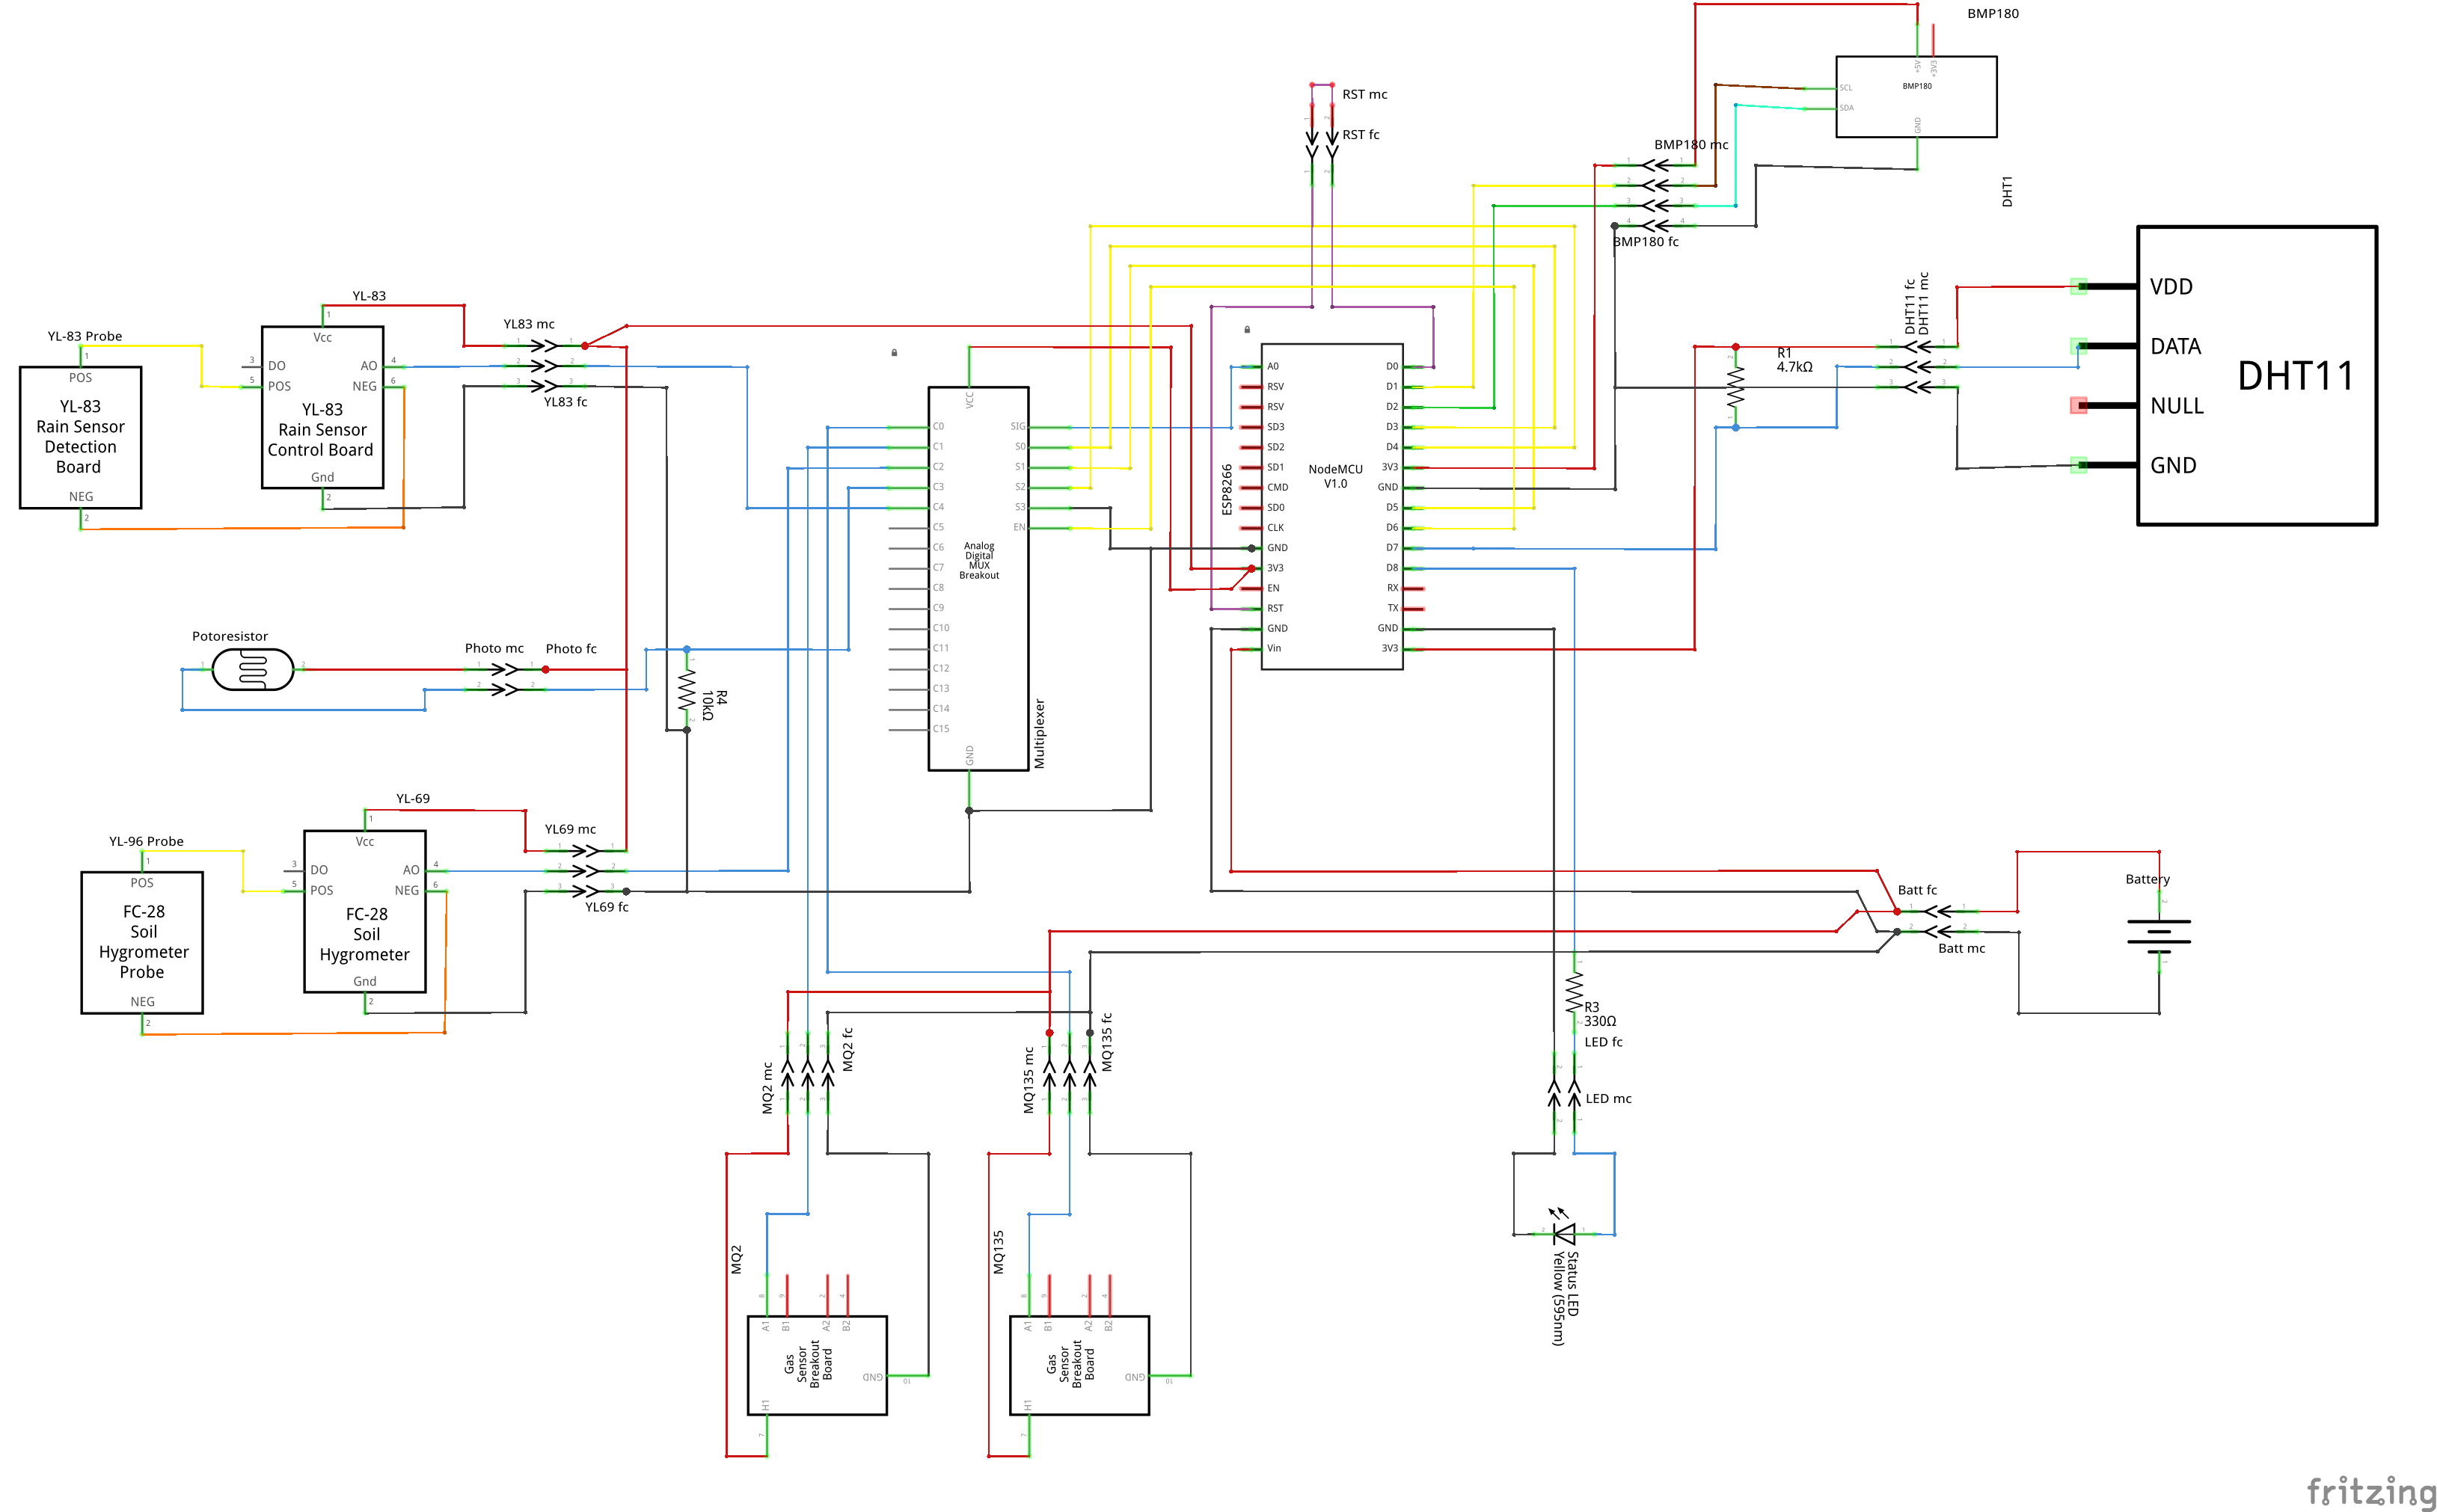
\includegraphics[scale=0.4]{hardware/iot_project_schem.png}
\caption{Schematica del cirtuito}
\label{fig:schematics}
\end{figure}

\begin{figure}[htbp]
\centering
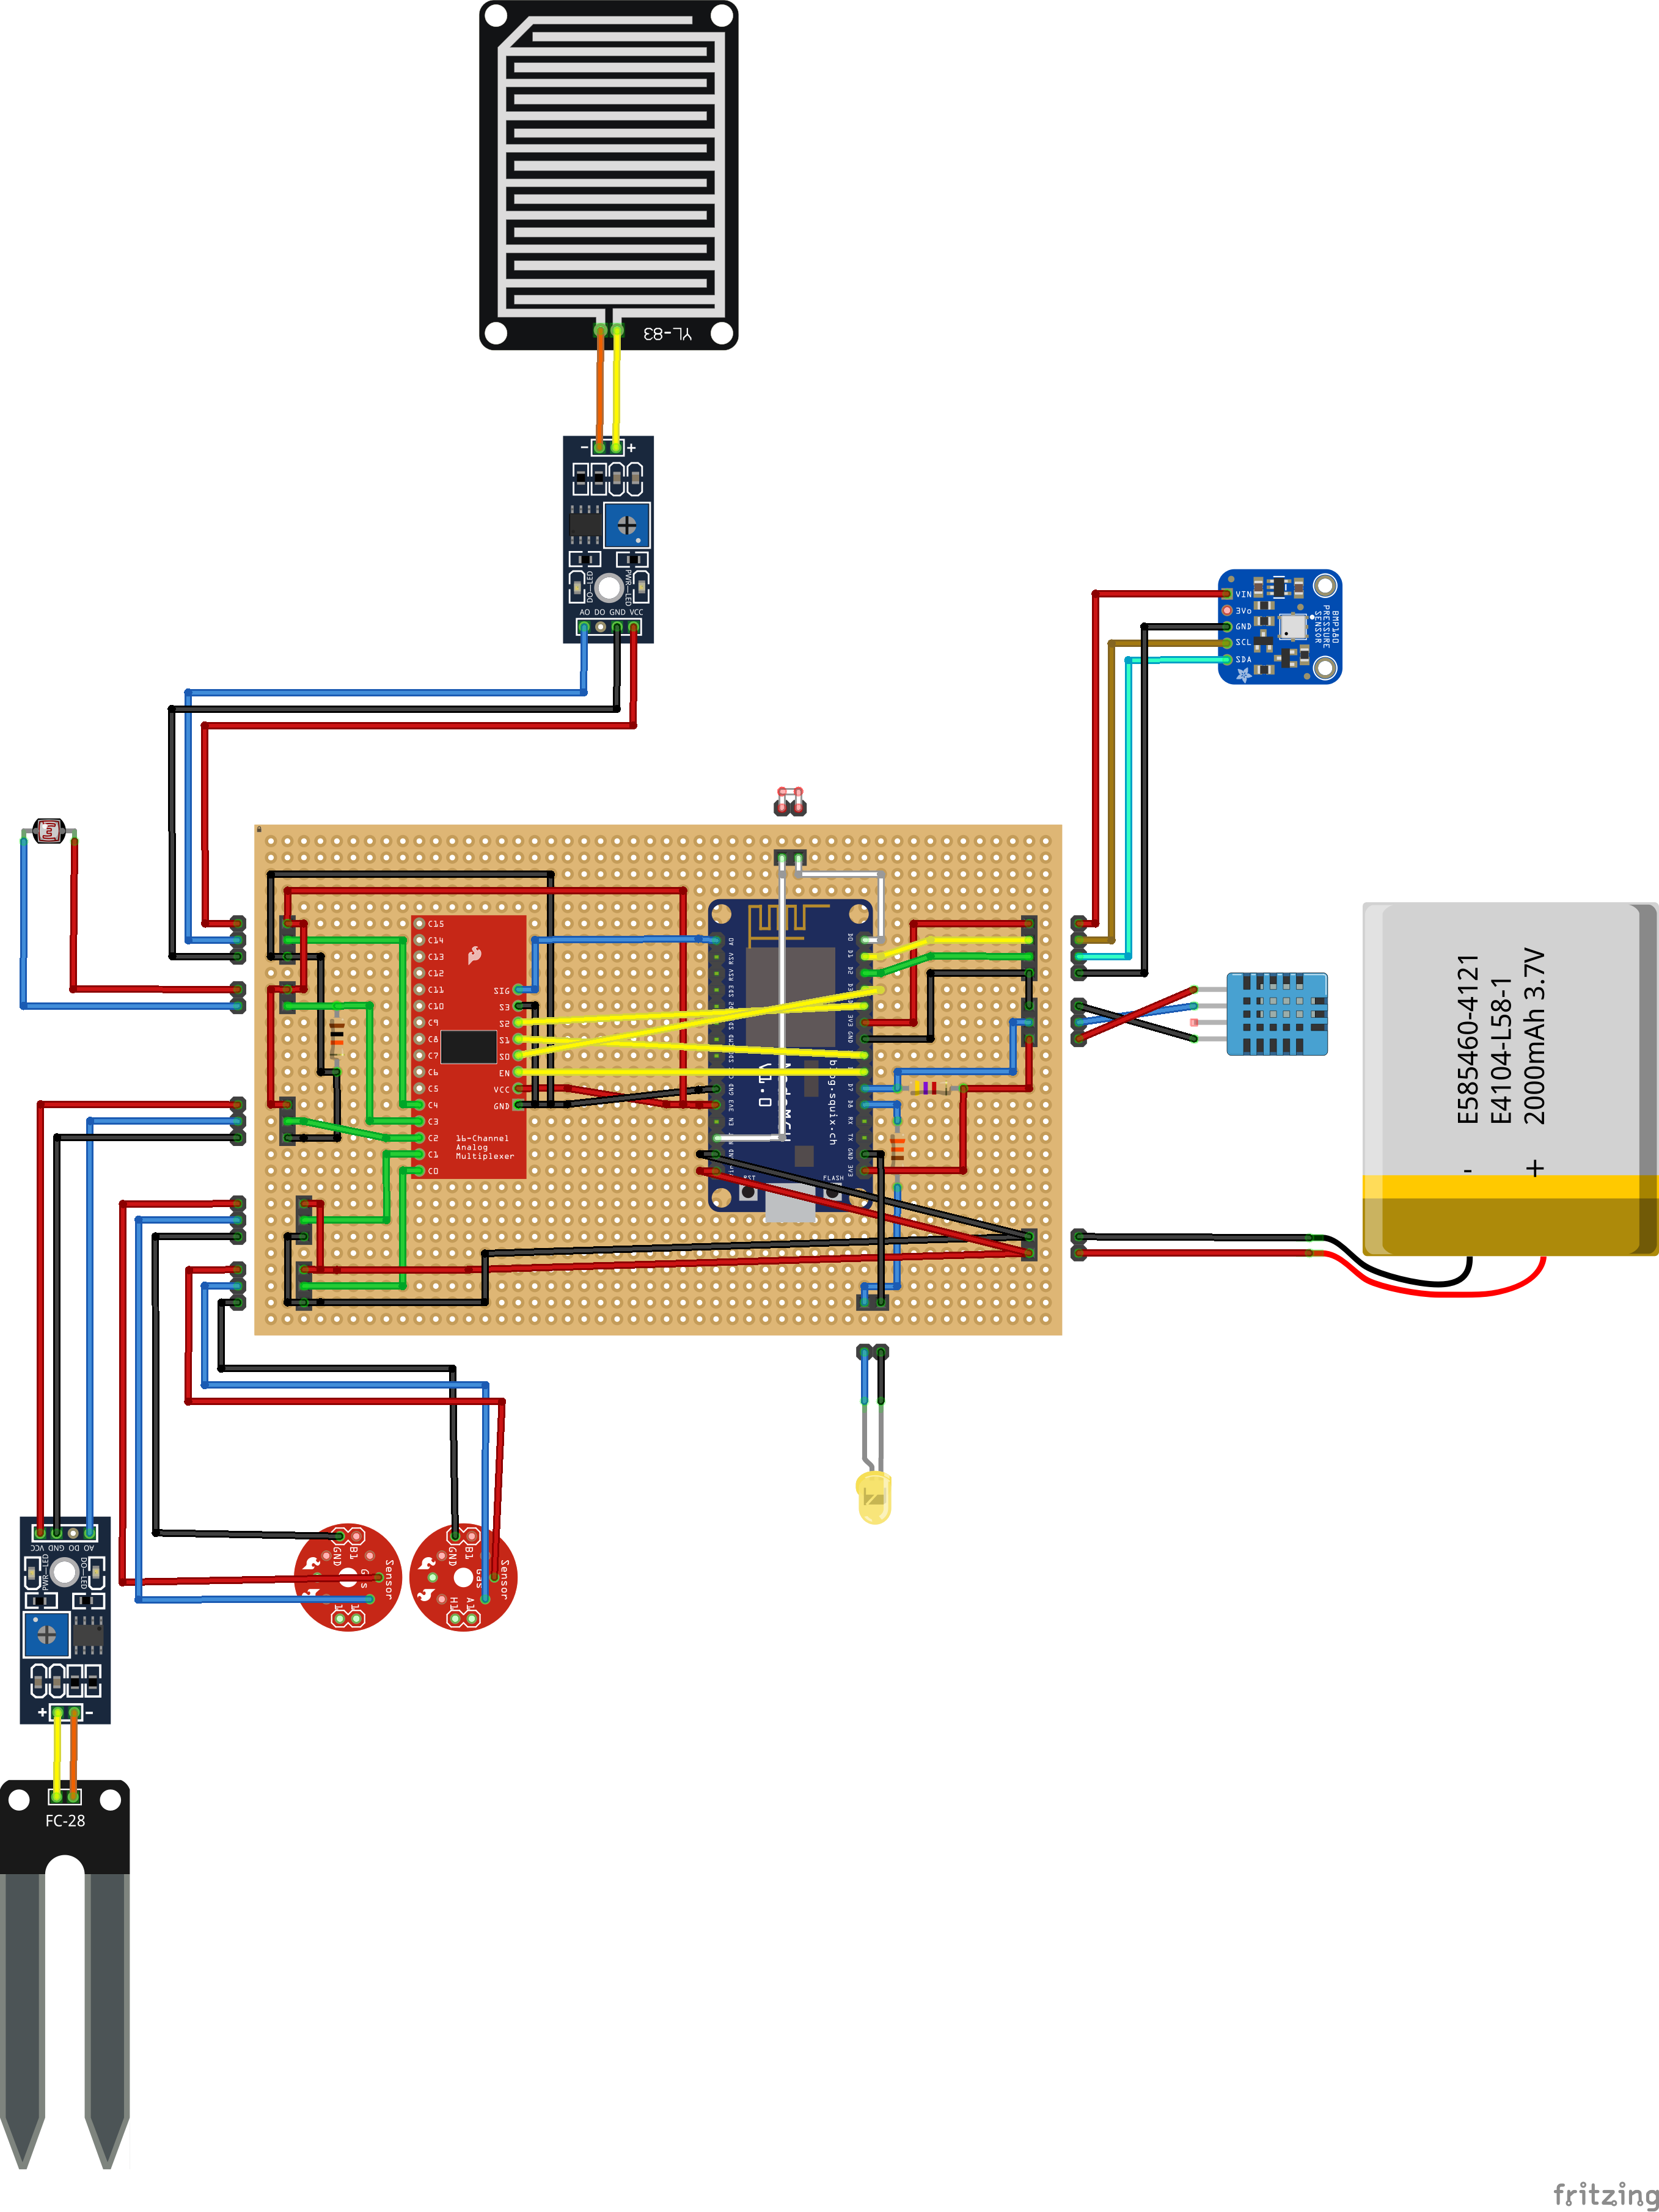
\includegraphics[scale=0.3]{hardware/iot_project_bb.png}
\caption{Schematica della breadbord}
\label{fig:breadboard}
\end{figure}

\begin{figure}[htbp]
  \centering
  \subcaptionbox{Vista della scatola}{\includegraphics[scale=0.25]{hardware/smart_box.pdf}}
  \subcaptionbox{Vista della scatola + supporto}{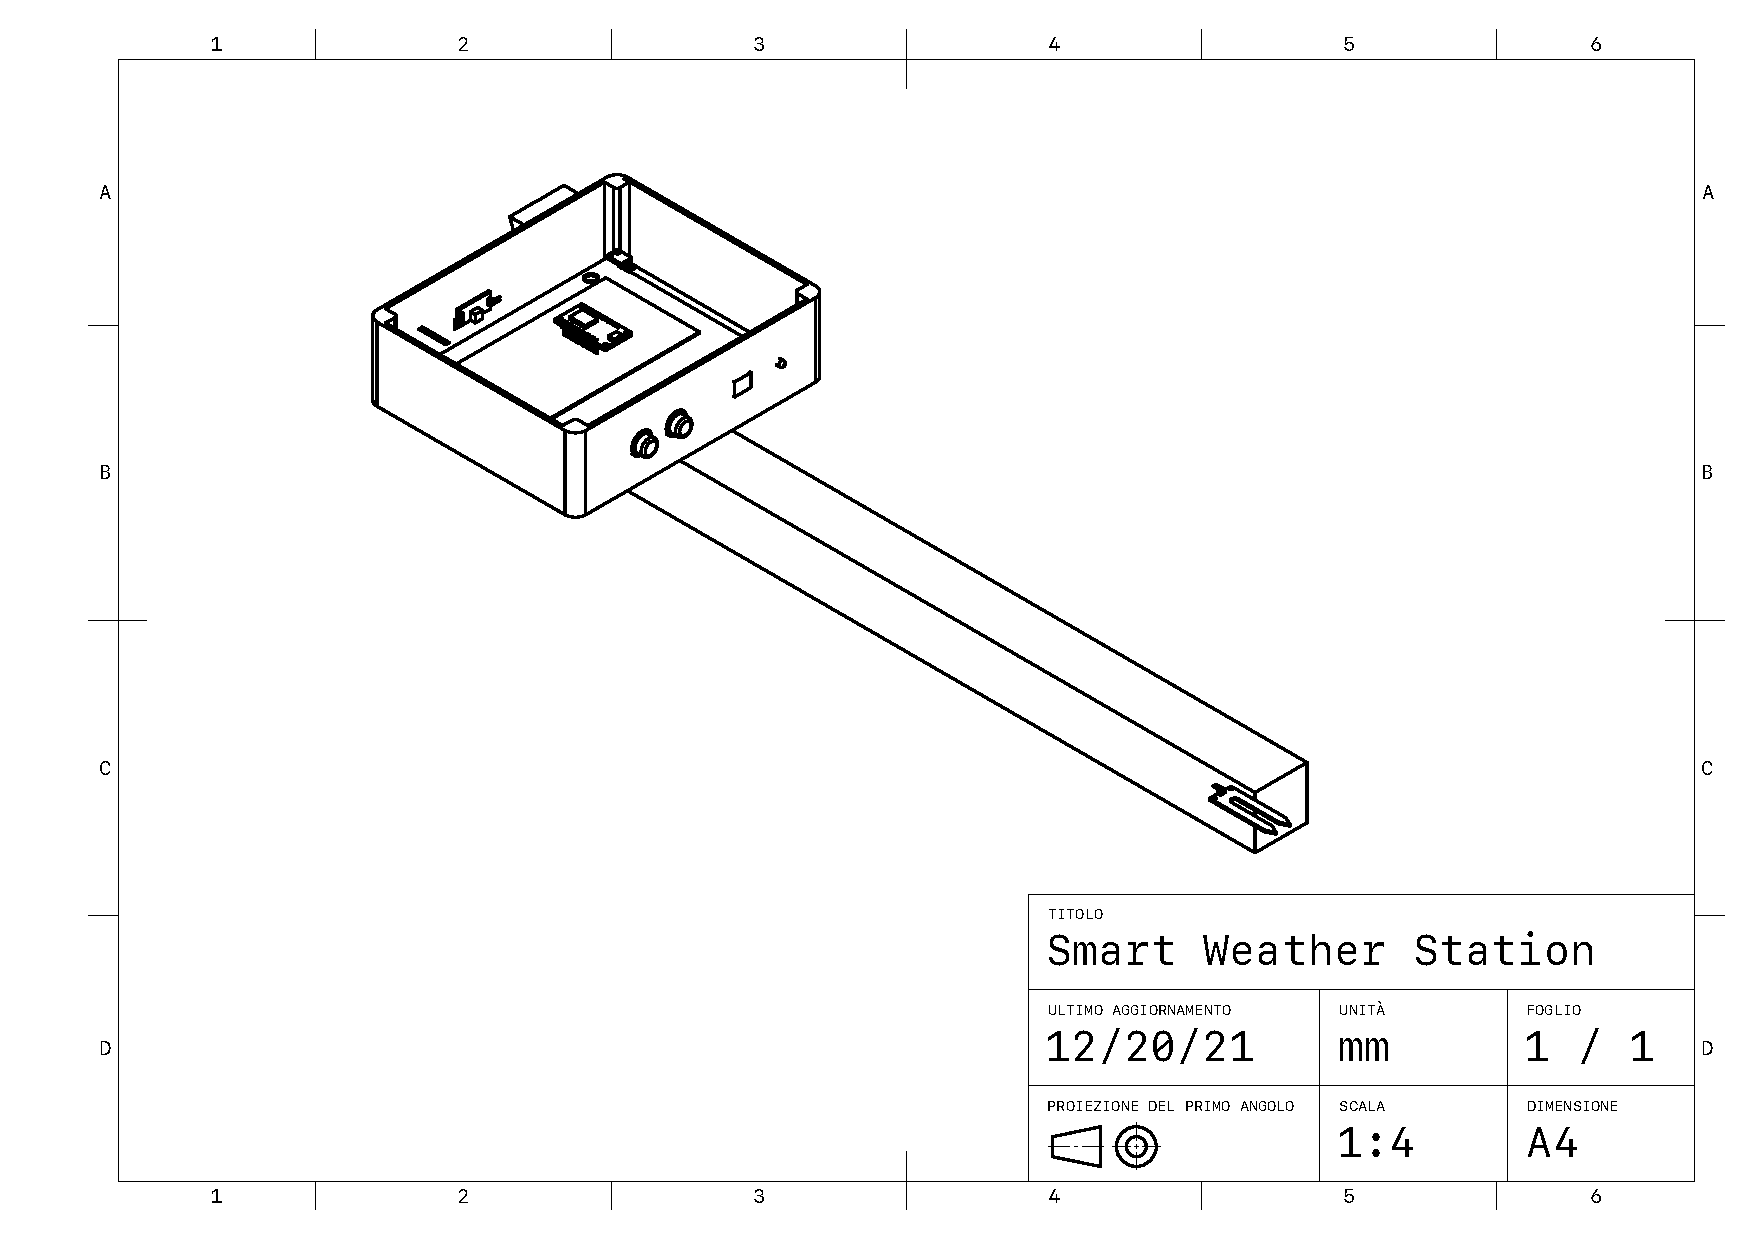
\includegraphics[scale=0.25]{hardware/smart_box_complete.pdf}}
  \caption{Modelli 3D della Smart Box}
  \label{fig:models}
\end{figure}

Oltre a questi due schemi è stato anche realizzato un modello 3D di tutti i componenti, compresa la scatola che li racchiude, per essere sicuri delle effettive misure di ogni componente e poter vedere come sarà il 
prodotto una volta terminato; i disegni in Figura \ref{fig:models} sono stati creati utilizzando lo strumento per la progettazione di modelli 3D Shapr3D. 

Una volta progettata la Smart Box si è passato alla fase di realizzazione, acquistati tutti i diversi componenti, gli schemi sono stati assemblati su una base millefori ottenendo il risultato in Figura \ref{fig:assembled}

\begin{figure}[htbp]
\centering
\includegraphics[scale=0.1]{hardware/photo/IMG_20220126_105605.jpg}
\caption{Circuito realizzato su breadboard}
\label{fig:assembled}
\end{figure}

\subsection*{Raccolta dei dati}
\vspace{0.5cm}

Per la raccolta dei dati generati dai sensori si è deciso di scrivere un programma utilizzando Arduino, popolare piattaforma open source per lo sviluppo di programmi eseguibili su microcontrollori, poiché 
integra nativamente tutte le librerie necessarie per interagire con i sensori e con l'ESP8266. 

Il programma, chiamato `collector.ino`, si connette alla rete WiFi preconfigurata ad ogni avvio dell'MCU, raccoglie i dati provenienti da ogni sensore in quell'instante di tempo e li invia ad un server InfluxDB 
etichettati in maniera appropriata, infine sfrutta la funzionalità dell'ESP8266 di Deep Sleep per mandare l'MCU in uno stato di sonno profondo per altri 15 minuti. In questo modo sia L'ESP che i sensori sono 
disattivati completamente (a parte un circuito interno all'ESP usato per il risveglio) riducendo al minimo il consumo di corrente.

Come detto precedentemente i dati raccolti dalla Smart Box sono caricati sul cloud utilizzando il servizio InfluxBD, un database open-source per serie temporali che offre strumenti di raccolta e analisi appositamente 
creati per gestire questo tipo di dato molto comune nell'ambiente IoT.

\begin{figure}[htbp]
\centering
\includegraphics[scale=0.1]{hardware/photo/IMG_20211222_112505.jpg}
\caption{Smart Box nella sua posizione finale}
\label{fig:inplace}
\end{figure}

Una volta realizzata la Smart Box si è deciso di posizionarla in una parte di giardino adibita ad orto nelle vicinanze di casa mia, Figura \ref{fig:inplace}, questo posto è perfetto poiché è molto simile ad un campo agricolo, 
inoltre è abbastanza vicino da collegarsi alla rete WiFi di casa senza aver bisogno di particolari antenne per estndere il segnale. 
Una volta nella sua posizione definitiva la raccolta dei dati può aver inizio; il periodo di raccolta va dal girono 23/12/2021 al giorno il 17/01/2022, per un totale di 25 giorni che, con la frequenza di un campione 
ogni 15 minuti, ha prodotto all'incirca 2400 campioni singoli.

\subsection*{Analisi dei dati}
\vspace{0.5cm}

\begin{table}
  \centering
\begin{tabular}{ l l l l l }
  sensore & media & std & mediana & moda (n.) \\
  \hline
  temperatura DHT11 & 6.17 & 4.69 & 6.0 & 4.0 (216) \\
  \hline
  temperature BMP180 & 5.87 & 6.29 & 4.9 & 4.5 (29) \\
  \hline
  humidità & 83.87 & 9.72 & 87.0 & 88.0 (856) \\
  \hline
  LDR \% & 38.08 & 46.91 & 0.0 & 0.0 (1319) \\
  \hline
  pioggia \% & 14.13 & 28.41 & 1.0 & 1.0 (1754) \\
  \hline
  igrometro \% & 53.42 & 15.81 & 57.0 & 58.0 (187) \\
  \hline
  MQ-135 \% & 8.32 & 1.65 & 8.0 & 8.0 (1672) \\
  \hline
  pressione & 96357.00 & 845.43 & 96376.0 & 95411.0 (6) \\
  \hline
  altitudine & 423.11 & 73.31 & 421.21 & 354.49 (7) \\
  \hline
\end{tabular}
\caption{ Valori statistici ricavati da ogni sesnore }
\label{tab:all_data_stats}
\end{table}

I dati raccolti sono stati elaborati con uno script python che ha calcolato per ogni sensore: media, deviazione standard, mediana e moda.
Guardando la Tabella \ref{tab:all_data_stats} possiamo scoprire diversi fenomeni interessanti: innanzitutto la temperatura media rilevata dal sensore DHT11 e quella rilevata da BMP180 sono molto simili, 
questo ci da conferma del corretto funzionamento dei due sensori.

Come seconda cosa notiamo che la media del sensore LDR è del 38\% poichè, essendo inverno durante il periodo di raccolta dati, ci sono state 
più ore di buio che di luce.

Analizzando il sensore di gas MQ-135 si nota che il suo valore medio, mediano e modale è all'incirca di 8\%, con una variazione del 1.6\%, questo indica che durante l'intero periodo di misurazione 
la qualità dell'aria è rimasta sempre all'incirca costante.

Se confrontiamo i valori ricavati dal sensore di pioggia con quelli dell'igrometro possiamo vedere come il valore medio sia del ~14\% inidcando che durante il periodo di misurazione ci sono pochi 
momenti di pioggia, inoltre la moda è dell'1\% con 1754 valori distinti. Confrontando i valori del sensore di pioggia con quelli dell'igrometro si può notare come a differenza 
della pioggia, il terreno ha un valore del ~53\%.

\begin{table}
  \centering
  \begin{tabular}{ l c c }
  sensore & media giorno & media notte \\
  \hline
  temperatura DHT11 & 8.71 & 4.55 \\
  \hline
  temperatura BMP180 & 9.90 & 3.31 \\
  \hline
  humidità & 80.08 & 86.27 \\
  \hline
  pioggia \% & 11.85 & 15.57 \\
  \hline
  igrometro \% & 53.50 & 53.37 \\
  \hline
  LDR \% & 96.29 & 1.14 \\
  \hline
  MQ-135 \% & 8.42 & 8.26 \\
  \hline
  pressione & 96418.27 & 96318.11 \\
  \hline
  altitudine & 417.81 & 426.47 \\
  \hline
  \end{tabular}
  \caption{A tab}
  \label{tab:daynight}
\end{table}

Un ulteriore analisi che si può svolgere è dividere l'intero dataset in campioni raccolti durante il giorno e quelli durante la notte filtrando i dati a seconda del valore di LDR. 
Otteniamo 919 campioni durante il girno (~39\%) e 1448 di notte (~61\%); la Tabella \ref{tab:daynight} riporta la media di per ogni sensore.

Si può vedere che la maggior parte dei sensori non avariano di molto fra notte e gironi, mentre temperatura, humidità, ldr cambiano radicalmente; come aspettato il valore medio 
del sensore di luminosità durante il giorno è ~96\% mentre durante la notte è ~1\%, stessa cosa avviene con la temperatura, che durante la notte è ~4°C, mentre di 
giorno aumenta fino a ~9°C. Il valore d'umidità invece aumenta di notte e diminuisce il giorno, in seguito approfondiremo queso fenomeno parlando della corelazione fra umidità e temperatura.

Una volta visti alcuni dati statistici di basesi vari valori si è deciso di calcolare alcune correlazioni fra di essi. Di seguito infatti si è deciso di calcolare la covarianza fra i valori di ogni sensore. 
> In statistica e in teoria della probabilità, la covarianza di due variabili statistiche o variabili aleatorie è un valore numerico che fornisce una misura di quanto le due varino assieme, ovvero della loro dipendenza.

In particolare si è calcolato prima l'indice di correlazione di Pearson e poi il coefficiente di correlazione di Spearman

> L'indice di correlazione R per ranghi di Spearman è una misura statistica non parametrica di correlazione. 
Essa misura il grado di relazione tra due variabili e l'unica ipotesi richiesta è che siano ordinabili, e, se possibile, continue. 
Diversamente dal coefficiente di correlazione lineare di Pearson, il coefficiente di Spearman non misura una relazione lineare anche qualora vengano usate misure intervallari. 
Infatti esso permette di stabilire quanto bene una relazione tra due variabili può essere descritta usando una funzione monotona.


%  | | temerature | humidity | rain_meter_percent | igrometer_percent | ldr_percent | mq135_percent | pressure |bmp_temperature| altitude |
%  | - | - | - | - | - | - | - | - | - |-|
%  | temerature | 1. | 0.28434172 | 0.00410613 | 0.22814114 | 0.43594109 | 0.45992467 | -0.01417428 | 0.96957958 | 0.01460149 |
%  | humidity | 0.28434172 | 1. | 0.2963187 | 0.19035885 | -0.18492689 | 0.38038485 | -0.36122921 | 0.23851606 | 0.36129079 |
%  | rain_meter_percent | 0.00410613 | 0.2963187 |  1. | -0.2540873 | -0.01087171 | 0.14955735| -0.54846696 | 0.03064852 | 0.54847466|
%  | igrometer_percent | 0.22814114 | 0.19035885| -0.2540873 | 1. | 0.05860886| -0.17551336| 0.35409045 |  0.19663955| -0.35407538|
%  | ldr_percent | 0.43594109 | -0.18492689| -0.01087171 | 0.05860886 | 1. | 0.06660318 | 0.08855831  | 0.52142574 |-0.08852001|
%  | mq135_percent | 0.45992467 | 0.38038485 | 0.14955735 |-0.17551336 | 0.06660318 | 1. | -0.19407299 | 0.44151245 | 0.19437162|
%  | pressure | -0.01417428 |-0.36122921 |-0.54846696 | 0.35409045 | 0.08855831| -0.19407299 |1. | -0.02541062| -0.99994044|
%  | bmp_temperature |  0.96957958 | 0.23851606 | 0.03064852 | 0.19663955 | 0.52142574 | 0.44151245| -0.02541062|  1. | 0.02577584|
%  | altitude |  0.01460149 | 0.36129079 | 0.54847466 |-0.35407538| -0.08852001|  0.19437162| -0.99994044 | 0.02577584|  1. |

Da questa tabella possiamo vedere molti valori interessanti.

La correlazione fra temperarua, temperatura del sensore mbp e percentuale di luce solare, come visto anche prima, e come si aspettava è abbastanza alta, ~0.45/~0.53 ed è una 
covarianza positiva, all'aumentare di una variabile, aumenta anche la seconda; questo poiché, come deddo in precedenza, durante il girno è intuitivo avere temperature più elevate rispetto che durante la notte.
Un'altra corelazione interessante è quella fra igrometro e sensore di pioggia, che controintuitivamente a quello che si può pensare è una covarianza negativa, all'aumntare 
della prima variabile, la seconda diminuisce, con un valore di ~-0.2, non molto, ma comunque non è trascurabile.    

\subsection*{Rilevazione anomalie}
\vspace{0.5cm}

\subsection*{Conclusione}
\vspace{0.5cm}

\end{document}